\chapter{甲状腺肿}

正常成人的甲状腺形似“H”,重量约20~30g,面积为20cm\textsuperscript{2}
左右,女性的甲状腺稍大略重于男性,触诊时不能触及。正常人甲状腺存在一定的变异,以峡部缺失及出现锥体叶最为常见。由于甲状悬韧带将甲状腺固着于喉及气管壁上,吞咽时甲状腺可随喉上下移动,作为判断甲状腺是否肿大以及判断颈部肿块是否与甲状腺有关的依据之一。甲状腺肿(goiter)系指甲状腺增大至正常大小2倍或以上者。

\section{【甲状腺肿大的检查步骤】}

\subsection{(一)病史询问}

甲状腺肿大的症状诊断主要包括病史采集、症状分析与综合判断。病史询问要了解是否来源于缺碘或高碘地区,有无碘摄入史、精神创伤史、手术史及头颈部放疗史;是否服用含碘药物或使用含碘造影剂等病史。有否代谢亢进或代谢减低的相应症状;有无眼部症状、神经精神症状。了解体重变化情况、有无食欲变化或腹泻等消化道症状。详细询问甲状腺(颈前)区有无疼痛、肿大及其特点与变化规律等。通过以上病史询问,应对患者的代谢情况进行初步的综合估计:是正常、亢进抑或减低。

\subsection{(二)甲状腺的体格检查}

应包括望诊、触诊与听诊:被检查者采取坐位,面向光源,头部稍向后仰,眼向前望,此时肿大的甲状腺形状较易显现。先观察其颈部有无手术瘢痕,若见颈前有肿大,被检查者应做吞咽动作或饮水一口,观察该肿物是否随吞咽而上下移动。若甲状腺肿应随吞咽动作上下移动,而非甲状腺组织则无此现象。但也有例外,如巨大的甲状腺肿、甲状腺癌、慢性侵袭性纤维性甲状腺炎等固着于甲状腺周围组织时,也可不随吞咽动作而上下移动。另外,舌后甲状腺肿者可在伸舌时于咽部窥见。而在有些消瘦明显的人,甲状腺腺体(尤其是峡部)比较突出,亦可被误认为甲状腺肿。

甲状腺肿的分度:一般将肿大的甲状腺分为三度,视诊不能确定甲状腺肿,触诊可扪及者为Ⅰ度;视诊可见甲状腺肿大,触诊可扪及,但肿大的甲状腺在胸锁乳突肌以内者为Ⅱ度;肿大的甲状腺超过胸锁乳突肌外缘者为Ⅲ度。

触诊甲状腺时,检查者站在患者的后方,以双手指柔和进行触诊。先应确认环状软骨的位置,甲状腺位于甲状软骨下紧贴在气管第三、四软骨环前面,由峡部连接着左右侧叶组成。触诊时注意甲状腺的大小、形状、性质,正常甲状腺质软如橡胶样感觉。弥漫性甲状腺肿伴甲状腺功能亢进症患者的甲状腺肿大,质地较正常者稍软;慢性淋巴性甲状腺炎者质稍硬,呈木样感觉;甲状腺癌或慢性侵袭性纤维性甲状腺炎者可硬如石头。同时还要注意甲状腺有无压痛、结节、血管震颤,与周围组织有无粘连,附近淋巴结情况以及有无气管移位等情况。甲状腺听诊有时可闻及血管杂音。

甲状腺肿的诊断有时还需与颈前部肿块进行区别:①颈前成堆脂肪组织:如有横亘于前颈甲状腺部位的成堆脂肪组织,其外形与质地颇似甲状腺肿,临床上常误诊为甲状腺肿,但做吞咽动作时并无上下移动;②甲状旁腺腺瘤或囊肿:甲状旁腺在甲状腺的2个侧叶后面,当甲状旁腺发生腺瘤或囊肿时,使甲状腺体隆起肿大,吞咽动作时也可上下移动,其表面光滑,质也坚韧,故甚似甲状腺肿大,仅从局部体征常不易鉴别,必须结合甲状旁腺功能亢进的临床表现。

\section{【甲状腺肿的分类】}

1.根据甲状腺肿的发生是否有区域聚集性,可分为地方性甲状腺肿(endemic
goiter)和散发性甲状腺肿(sporadic goiter)。

2.根据甲状腺肿是否存在结节,分为结节性甲状腺肿(nodular
goiter)和弥漫性甲状腺肿(diffuse goiter)。

3.根据甲状腺肿是否伴有功能亢进,分为毒性甲状腺肿(toxic
goiter)和非毒性甲状腺肿(nontoxic goiter)。

此外,甲状腺肿的诊断还需区分肿大的甲状腺是否伴有疼痛,如痛性甲状腺肿常见于急性化脓性甲状腺炎、亚急性甲状腺炎;甲状腺癌如侵犯或压迫神经也可引起疼痛;其他原因的甲状腺肿一般无疼痛。结节性甲状腺肿又可为单个(单发性)或多个(多发性)。

甲状腺肿的质地和形态:甲状腺肿大可分为弥漫型、结节型和混合型。单纯性甲状腺肿、甲状腺功能亢进症、亚急性甲状腺炎、慢性淋巴性甲状腺炎者多数呈弥漫性对称性肿大,并保持正常的甲状腺外形,除了慢性淋巴性甲状腺炎的质地较坚硬外,一般腺体的质地较软;结节型单纯性甲状腺肿、结节性甲状腺功能亢进症、甲状腺腺瘤、甲状腺癌、慢性侵袭性纤维性甲状腺炎等则呈不规则的或局限性甲状腺肿;甲状腺腺瘤的轮廓清楚,表面平滑呈球形,触之有弹性感,而甲状腺癌则较硬实、表面不平滑。

甲状腺肿的病因:一旦确定为甲状腺肿,应进一步检测其功能是否正常(euthyroid)、亢进(hyperthyroidism)或者减退(hypothyroidism),继而寻找出病因(表\ref{tab38-1})。

\section{【甲状腺功能的检查】}

\subsection{(一)血清甲状腺激素水平}

反映甲状腺功能的血清激素包括总三碘甲状腺原氨酸(TT\textsubscript{3}
)、总甲状腺素(TT\textsubscript{4}
),游离三碘甲状腺原氨酸(FT\textsubscript{3}
)和游离甲状腺素(FT\textsubscript{4}
),它的异常说明已经存在显性甲状腺功能的病变。血清T\textsubscript{3}
、T\textsubscript{4}
受到甲状腺激素球蛋白(TBG)浓度的影响,FT\textsubscript{3}
、FT\textsubscript{4}
直接反映活性甲状腺激素(生物效应的主要部分),且不受TBG的影响,更准确反映甲状腺的功能状态,是目前临床甲状腺功能的疾病诊断、病情判断、疗效观察最常用的指标。

\subsection{(二)下丘脑-垂体-甲状腺功能轴}

\subsubsection{1.血清促甲状腺激素(TSH)的测定}

随着检测技术水平的发展,TSH测定方法在灵敏度上有大幅度提高,在T\textsubscript{3}
、T\textsubscript{4}
变化之前TSH(超敏TSH,uTSH)已经改变了。使TSH在人群中进行甲状腺功能筛查时,能更有效地筛查出甲亢,尤其是亚临床甲亢的异常,是反映甲状腺功能的最敏感的指标。

\begin{table}[htbp]
\centering
\caption{甲状腺肿按其功能分类}
\label{tab38-1}
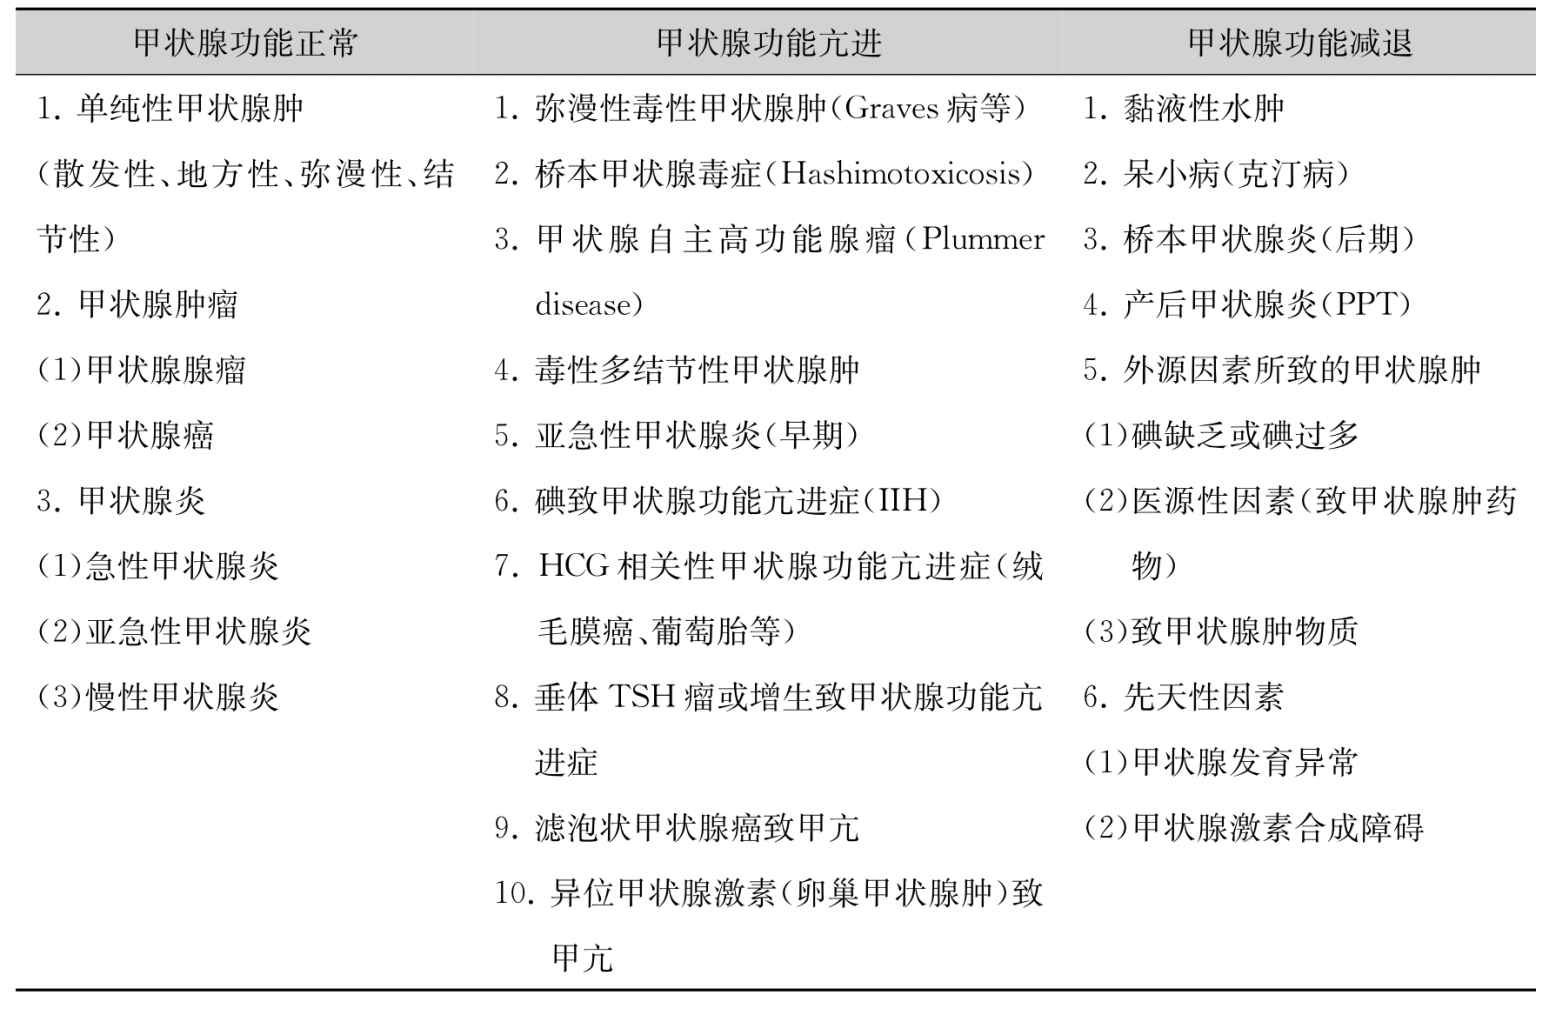
\includegraphics[width=5.92708in,height=3.875in]{./images/Image00238.jpg}
\end{table}

\subsubsection{2.促甲状腺激素释放激素(TRH)兴奋试验}

反映垂体TSH分泌细胞的储备功能和对TRH的敏感性。临床上可作为甲亢或甲减的病因鉴别诊断。

\subsection{(三)甲状腺自身抗体的检测}

\subsubsection{1.甲状腺过氧化物酶抗体(TPOAb)}

TPOAb是自身免疫性甲状腺疾病(AITD)的标志性抗体,是诊断桥本甲状腺炎的金标准。虽然不是AITD的诱因或致病始动因子,但它反映着甲状腺自身免疫状态的存在,但与AITD的严重程度并没有直接的关系。

\subsubsection{2.甲状腺球蛋白抗体(TgAb)}

TgAb也是AITD的标志性抗体,往往伴随TPOAb同时出现。甲状腺球蛋白(Tg):反映甲状腺滤泡是否破坏的指标。

\subsubsection{3.TSH受体抗体(TRAb)}

是自身免疫性甲状腺疾病的病因,包括TSH受体刺激性抗体(TSAb)、TSH刺激阻断性抗体(TSBAb)和TSH受体结合抑制免疫球蛋白(TBII)。狭义的TRAb仅指TBII,临床上通常测定TBII代替TSAb。TSAb可作为判断Graves病的进展或预测复发的作用,以及治疗后停药的重要指标。

\subsection{(四)放射性核素的甲状腺功能和显像检查}

主要包括\textsuperscript{131}
碘摄取率和甲状腺核素静态显像,随着甲状腺激素特别是TSH测定方法的进步,\textsuperscript{131}
碘摄取率已经不再作为诊断甲亢和甲减的常规指标。目前主要用于甲亢所致的甲状腺毒症和炎症所致的甲状腺毒症的鉴别诊断。甲状腺核素静态显像主要用于甲状腺结节和肿瘤的诊断和鉴别诊断。

\subsubsection{1.甲状腺\textsuperscript{131} I摄取率}

应用范围包括:①计算\textsuperscript{131}
I治疗甲亢时需要的活度;②Graves病和破坏性甲状腺毒症(如亚急性甲状腺炎、产后甲状腺炎等)所致的高甲状腺激素血症的鉴别病因。亚急性甲状腺炎因甲状腺滤泡遭受炎性破坏而出现甲状腺摄\textsuperscript{131}
I能力明显减低,同时有FT\textsubscript{3} 、TT\textsubscript{3}
、FT\textsubscript{4} 、TT\textsubscript{4}
升高以及TSH减低,呈摄\textsuperscript{131}
I能力与血清甲状腺激素水平分离现象;③非毒性甲状腺肿与Graves病的鉴别,前者甲状腺摄\textsuperscript{131}
I率因缺碘可升高,但高峰不前移,后者高峰前移。

\subsubsection{2.甲状腺核素静态显像}

通过显像可显示甲状腺位置、大小、形态及放射性分布状况,以及了解甲状腺结节和肿瘤的局部功能状态。正常甲状腺图像:甲状腺双叶呈蝴蝶状,叶内放射性分布均匀,双叶上极因甲状腺组织较薄,放射性分布略有些稀疏,峡部一般不显像或其浓集程度明显低于双侧甲状腺叶,偶尔可见到锥状叶。根据甲状腺结节摄取核素能力的不同可分为“热结节”、“温结节”和“冷结节”,可为结节的鉴别诊断以及异位甲状腺组织的诊断提供信息。

\paragraph{(1)热结节:}

是结节组织摄取核素能力高于周围正常甲状腺组织,在结节部位出现放射性浓集,常见于自主功能性甲状腺结节(或腺瘤)。其显像特点甲状腺失去正常形态,在甲状腺解剖部位见到一个放射性浓集区(一般为圆形或类圆形),对侧叶未见显像或显像模糊。热结节病理上多为良性自主性腺瘤,甲状腺癌罕见。

\paragraph{(2)温结节:}

指结节组织摄取核素能力与周围正常甲状腺组织相近,使得结节的放射性分布与周围正常甲状腺组织无明显差异。它的显像特点双侧叶内核素分布均匀,未见到明显的核素分布稀释区或浓集区。温结节属功能正常,常见于甲状腺腺瘤;也可见于甲状腺癌,多为分化好的甲状腺癌。

\paragraph{(3)冷结节:}

结节部位对核素的摄取能力低于周围正常甲状腺组织,因此该部位出现核素分布稀疏区或缺损区。显像特点为甲状腺肿大,形态不完整,其中一叶内可见单一核素分布稀疏区或缺损区,对侧叶核素分布均匀。冷结节是甲状腺腺瘤常见的显像类型,还见于甲状腺囊肿、囊性变、出血、钙化、结节性甲状腺肿、甲状腺炎、甲状腺癌等。在冷结节中,甲状腺癌约占5\%~10\%。

\paragraph{(4)甲状腺亲肿瘤核素显像:}

在甲状腺静态显像显示肿瘤部位为核素分布稀疏区或缺损区,可再注射亲肿瘤显像剂。若此区域出现核素填充现象时,视为亲肿瘤显像阳性,提示该肿瘤恶性病变的可能性较大。不同类别的亲肿瘤显像剂阳性提示着不同类型的甲状腺癌,\textsuperscript{201}
Tl、\textsuperscript{99m}
Tc-MIBI显像阳性提示甲状腺分化癌(DTC),其特异性为80\%~90\%,少部分良性结节也可以显像阳性;\textsuperscript{99m}
Tc-二巯基丁二酸(DMSA)显像阳性提示甲状腺髓样癌,其灵敏度>80\%,特异性100\%;\textsuperscript{99m}
Tc-奥曲肽和\textsuperscript{131}
I-间位碘代卞胍(MIBG)可用于甲状腺髓样癌的诊断。

\subsection{(五)甲状腺CT和MRI}

可清晰显示甲状腺和甲状腺与周围组织器官的关系,对甲状腺结节的鉴别诊断有较高价值。当疑诊甲状腺癌时,CT和MRI能了解病变的范围、对气管的侵犯程度以及有无淋巴结转移等;还可以了解胸腔内甲状腺情况,区别甲状腺和非甲状腺来源的纵隔肿瘤。

\subsection{(六)甲状腺超声检查}

随着高分辨率超声显像技术的应用,超声检查可以测量甲状腺的大小,显示其形态是否规则,包膜是否光整,结构是否均匀,内有无结节以及结节的数量、大小、形态、物理性质等。彩色多普勒血流图(CDFI)可展现甲状腺整体及各部的血供情况以推断其功能状态。检查报告应包括结节的位置、形态、大小、数目、结节边缘状态、内部结构、回声形式、血流状况和颈部淋巴结情况。

\subsection{(七)甲状腺细针穿刺和细胞学检查(FNAC)}

FNAC主要用于甲状腺结节的鉴别诊断,分辨良、恶性病变。此外,它诊断慢性淋巴细胞性甲状腺炎和亚急性甲状腺炎也有很高特异性。FNAC结果:①良性病变(占70\%);②恶性病变(占5\%~10\%);③疑似恶性病变;④大约有5\%~15\%是因为标本取材不满意而不能诊断的。超声检查指导下FNAC的指征:触诊不满意的小结节;对囊性和实体性的混合性结节,为确保在实质性部分取样。怀疑结节恶性变者均应进行FNAC检查,手术前FNAC检查有助于术前明确癌症的细胞学类型,制订正确的手术方案。

\protect\hypertarget{text00298.html}{}{}

\section{126 功能性甲状腺肿}

\subsection{一、单纯性甲状腺肿}

非炎症和非肿瘤原因引起的不伴甲状腺功能异常的甲状腺肿,称为单纯性甲状腺肿(simple
goiter),可分为地方性和散发性甲状腺肿。当患病率超过10\%时,称为地方性甲状腺肿。地方性甲状腺肿的主要原因是碘缺乏,多见于山区或远离沿海的地区。散发的甲状腺肿约占人群的5\%,女性发病率是男性的3~5倍,散发性甲状腺肿的原因复杂,碘过量、致甲状腺肿物质以及激素合成障碍等。

\subsubsection{(一)甲状腺肿大特征}

单纯性甲状腺肿可分为弥漫型、结节型及混合型肿大。整个腺体滤泡增生、增大并富含胶质,多数为弥漫性肿大,质地柔软,表面光滑,无压痛,甲状腺常呈轻、中度肿大;部分为重度肿大。结节性甲状腺肿可见结节、纤维化、出血和钙化,表面可及结节。另有少数患者为混合型,甲状腺肿大伴有结节。

\subsubsection{(二)诊断依据}

\paragraph{1.症状}

甲状腺轻度肿大时无明显症状,中、重度肿大有不同程度的压迫症状,如肿物压迫而引起颈肿胀感、气促、声音嘶哑或吞咽困难等不适。胸骨后甲状腺肿可压迫头颈部和上肢静脉回流受阻。若合并甲状腺囊肿出血,可发生突然疼痛及腺体急骤增大。部分患者后期可出现甲状腺功能减退或者甲状腺功能亢进的症状。

\paragraph{2.地方性甲状腺肿}

是碘缺乏病(IDD)的主要表现之一,碘缺乏时合成甲状腺激素不足,反馈引起垂体分泌过量的TSH,刺激甲状腺增生肥大。长期的非毒性甲状腺肿可以发展为毒性甲状腺肿。甲状腺肿的患病率和甲状腺体积随着碘缺乏程度的加重而增加,补充碘剂后,甲状腺肿的患病率显著下降。部分轻度碘缺乏的人在机体碘需要增加的情况下可出现甲状腺肿,如青春期、妊娠期、哺乳期等。

\paragraph{3.散发性甲状腺肿}

除了外源性因素致甲状腺肿外(见下述),可能与甲状腺生长免疫球蛋白(thyroid
growth
immunoglobulins,TGI)相关:TGI是另一类作用在TSH受体的不同结合位点,它仅仅是刺激甲状腺细胞增生肿大,并不促进甲状腺激素的合成和释放,其生物效应与TSAb不同。内源性因素还包括先天甲状腺激素合成障碍,主要有甲状腺内的碘转运障碍、过氧化物酶活性缺乏、碘化酪氨酸偶联障碍、异常甲状腺蛋白形成、甲状腺球蛋白水解障碍、脱碘酶缺乏等,部分患者发生甲状腺功能减退(呆小病)。先天性甲状腺功能减退伴神经性耳聋称为Pendred综合征。

\paragraph{4.实验室检查}

血清T\textsubscript{3} 、T\textsubscript{4} 正常,T\textsubscript{4}
/T\textsubscript{3}
的比值常增高,血清TSH一般正常,甲状腺自身抗体基本正常。血清甲状腺球蛋白(Tg)水平增高,增高的程度与甲状腺肿的体积呈正相关。尿碘中位数(MUI)<100μg/L提示缺碘,有助于地方性甲状腺肿的诊断。甲状腺扫描:早期放射性分布均匀,晚期放射性分布不均。

\subsubsection{(三)外源性因素致甲状腺肿}

\paragraph{1.致甲状腺肿物质}

在食物中也有一些蔬菜,如卷心菜、木薯以及含氟过多的饮水等,因含有致甲状腺肿物质或抑制甲状腺合成的物质,均能阻止甲状腺浓聚碘或使酪氨酸不能碘化而引起甲状腺代偿性肿大。

\paragraph{2.药物}

致甲状腺肿的化合物种类很多,大多数属于硫代酰胺类(thioamides)与苯胺类,通过干扰碘的利用,阻止甲状腺激素合成而引起甲状腺肿。药物如硫脲类(甲巯咪唑)、对氨水杨酸、碳酸锂、保泰松等能阻止甲状腺激素的合成。硫氰酸盐、过氯酸盐、硝酸盐等能与碘竞争进入甲状腺而抑制碘的摄取。

\paragraph{3.碘缺乏或高碘}

正常人每日需合成甲状腺素100μg,最低需碘量65μg/d,当每日摄入碘量少于50μg就可发生甲状腺肿。机体缺碘时,不能合成足够的甲状腺激素,反馈引起垂体TSH的分泌增加,刺激甲状腺增生肿大。在青春期、妊娠期、哺乳期、寒冷、感染、创伤等刺激时,体内对甲状腺激素的需要量增多,可诱发或加重甲状腺肿。高碘致甲状腺肿主要为常年饮用含碘高的水,当碘摄入过多使碘的有机化过程受阻,甲状腺代偿性肿大。高碘的甲状腺肿较缺碘的甲状腺肿质感硬实之外,其尿碘浓度也比较高。

\protect\hypertarget{text00299.html}{}{}

\subsection{二、Graves病}

甲状腺功能亢进症(hyperthyroidism,甲亢)是指甲状腺腺体产生过多的甲状腺激素而引起的甲状腺毒症,其病因包括弥漫性毒性甲状腺肿(Graves病)、毒性结节性甲状腺肿、甲状腺自主性高功能腺瘤(Plummer
disease)。Graves病是甲状腺功能亢进症中最多见的,占所有甲亢的85\%左右。它与慢性淋巴细胞性甲状腺炎和产后甲状腺炎同属于自身免疫性甲状腺疾病(autoimmune
thyroid
disease,AITD),一种器官特异性自身免疫疾病。Graves病是以遗传为背景,在食物中的碘含量、感染、药物、精神刺激等环境因素作用下,诱发体液免疫和细胞毒性T淋巴细胞及细胞因子等参与下的免疫功能紊乱,导致甲状腺肿大、甲状腺功能亢进的临床综合征。

\subsubsection{(一)临床表现}

甲状腺毒症:①高代谢综合征:甲状腺激素分泌增多导致交感神经兴奋性增高和新陈代谢加速,患者常伴有怕热多汗、皮肤暖湿、多食善饥、体重显著下降、疲乏无力等;②精神神经系统:紧张焦虑、烦躁易怒、紧张激动、失眠不安、舌手细震颤;③心血管系统:心悸气促、心动过速(静息时仍快)、脉压增大;甲亢患者出现心律失常(房性期前收缩、心房颤动多见)、心脏增大、心力衰竭;④消化系统:食欲亢进,大便稀溏、次数增加;重者肝功异常;⑤肌肉骨骼系统:以甲亢周期性瘫痪(TTP)为主,20~40岁亚洲男性多发;诱因包括:剧烈运动、高碳水化合物饮食、应用胰岛素等;病变主要累及下肢、伴有低钾血症;TTP病程呈自限性,控制甲亢可以自愈;部分患者发生甲亢性肌病、眼肌麻痹,少数则伴发重症肌无力。也有发生胫前皮肤的黏液性水肿;⑥造血系统:血白细胞总数减低、淋巴细胞比例增加、单核细胞增加;⑦生殖系统:女性月经减少或闭经;男性阳痿。

\subsubsection{(二)甲状腺肿}

甲状腺的两叶多数呈弥漫性、基本对称性、不同程度的肿大,亦有部分患者不出现甲状腺肿。肿大的甲状腺质地较软,有充实感,表面通常是光滑的,可随吞咽上下移动;部分患者可触及结节。甲状腺的上下极可触及震颤,闻及血管杂音。

\subsubsection{(三)眼征}

Graves病的眼征颇为特别,其突眼程度与甲亢病情轻重无明显关系。分为2种类型:非浸润性和浸润性,任何病因的甲亢患者都可有眼睑挛缩、眼裂增宽的非浸润性眼征。眼睑挛缩改变了患者的外貌,常伴随有眼睛刺激症状。

\subsubsection{(四)实验室检查}

主要包括三大类:甲状腺激素、甲状腺自身抗体和甲状腺的影像学检查。

\paragraph{1.血清甲状腺激素水平}

血清T\textsubscript{3} 、T\textsubscript{4} 和FT\textsubscript{3}
、FT\textsubscript{4}
增高,其异常说明已经存在显性的甲状腺功能病变,尤其是FT\textsubscript{3}
、FT\textsubscript{4}
增高是诊断临床甲亢的首选指标。几乎所有甲亢和亚临床甲亢患者,血清TSH浓度都降低。TSH对突眼的鉴别诊断尤为重要,特别是对突眼出现在甲亢前的患者,当甲状腺激素水平还没有变化,如若TSH浓度降低,高度提示为甲状腺相关眼病。

\paragraph{2.甲状腺自身抗体}

在初发的Graves病患者血中,70\%~95\%可检测到TRAb

(TSAb);TSAb可用于甲状腺毒症的鉴别诊断,如亚急性甲状腺炎、无痛性或产后甲状腺炎和毒性结节性甲状腺肿,TSAb均为阴性。弥漫性毒性甲状腺肿(GD)患者血中的TPOAb阳性率约70\%~80\%,而TGAb阳性率为50\%左右。

\paragraph{3.甲状腺的影像学检查}

\subparagraph{(1)\textsuperscript{131} I摄取率:}

甲亢时\textsuperscript{131}
I的总摄取量增加,摄取高峰前移。目前主要用于甲状腺毒症病因的鉴别:甲亢所致的甲状腺毒症\textsuperscript{131}
I摄取率增高;非甲亢类型所致的甲状腺毒症\textsuperscript{131}
I摄取率减低。

\subparagraph{(2)甲状腺放射性核素扫描:}

主要用于鉴别甲状腺毒症的病因,Graves病的放射性核素扫描可见核素均质性的分布增强;结节性毒性甲状腺肿者则见核素分布不均,增强和减弱区呈灶状分布;甲状腺高自主功能腺瘤仅在肿瘤区有核素增强,其他区域的核素分布稀疏。

\subparagraph{(3)甲状腺超声:}

甲状腺呈弥漫性、对称性、均匀性增大(2~3倍),边缘多规则,内部回声多呈密集、增强光点,分布不均匀,部分有低回声小结节状改变。CDFI甲状腺腺体内血流呈弥漫性分布,血流量大,速度增快,血流量为正常人的8~10倍,彩色血流信号呈五彩缤纷状,即“火海征”。

\subsubsection{(五)鉴别诊断要点}

典型的Graves病诊断并不困难,根据甲状腺肿大、突眼征和心动过速等临床特征,作出诊断。但部分不典型病例或发病初期症状较轻者,单凭某些症状则不易判断,如以神经应激性增高症状为主要表现的易误诊为神经症;以胃肠道症状为主要表现的易误诊为慢性腹泻或结肠炎;以心律失常、心力衰竭为主要表现者易误诊为心脏疾病(尤其在老年人)等等。还有一些特殊类型的甲亢,如:甲状腺危象、淡漠型甲亢、亚临床甲亢、妊娠期甲亢、甲状腺功能亢进性心脏病、甲亢性周期性瘫痪、Graves眼病以及胫前黏液性水肿等,以某些突出的临床表现而易误诊为其他的相关疾病。另外,少数发生异位甲状腺(如胸骨后甲状腺、卵巢甲状腺、舌根后部甲状腺)者,如有明显的甲亢临床表现,但体检却未发现甲状腺肿大时,应考虑是否有异位。由于不典型的甲亢病例颇易误诊,临床有疑诊时必须依靠相关的甲状腺功能检测以作出诊断。

Graves病还应与引起甲状腺毒症的疾病进行鉴别:有甲状腺毒症表现而\textsuperscript{131}
I摄取率降低的是破坏性甲状腺毒症(如亚急性甲状腺炎、无痛性甲状腺炎),以及碘甲亢和伪甲亢(外源性甲状腺激素摄入过多所致甲亢)的特征。①典型亚急性甲状腺炎常有发热、颈部疼痛,早期T\textsubscript{3}
、T\textsubscript{4} 水平增高而\textsuperscript{131}
I摄取率低的“分离现象”,在甲状腺毒症期过后可有一过性甲减,之后甲状腺功能恢复正常;②无痛性甲状腺炎是自身免疫甲状腺炎的一个亚型,大部分患者要经历一个由甲状腺毒症至甲减的过程,然后甲状腺功能恢复正常,甲状腺肿大但不伴疼痛;③如果怀疑服用过多甲状腺激素引起的甲状腺毒症时,常可询问出过多使用甲状腺激素的病史,还可通过测定血中Tg水平进行鉴别,外源性甲状腺激素引起的甲亢Tg水平很低,而甲状腺炎者的Tg水平明显升高;④桥本甲状腺毒症(Hashitoxicosis)有甲亢的临床表现和实验室检查结果,且TPOAb和TgAb滴度高,少数患者可为一过性甲状腺毒症。单纯性甲状腺肿与甲状腺功能亢进的鉴别参见表\ref{tab38-2}。甲状腺毒症的病因鉴别见表\ref{tab38-3}。

\begin{table}[htbp]
\centering
\caption{单纯性甲状腺肿与Graves病的鉴别}
\label{tab38-2}
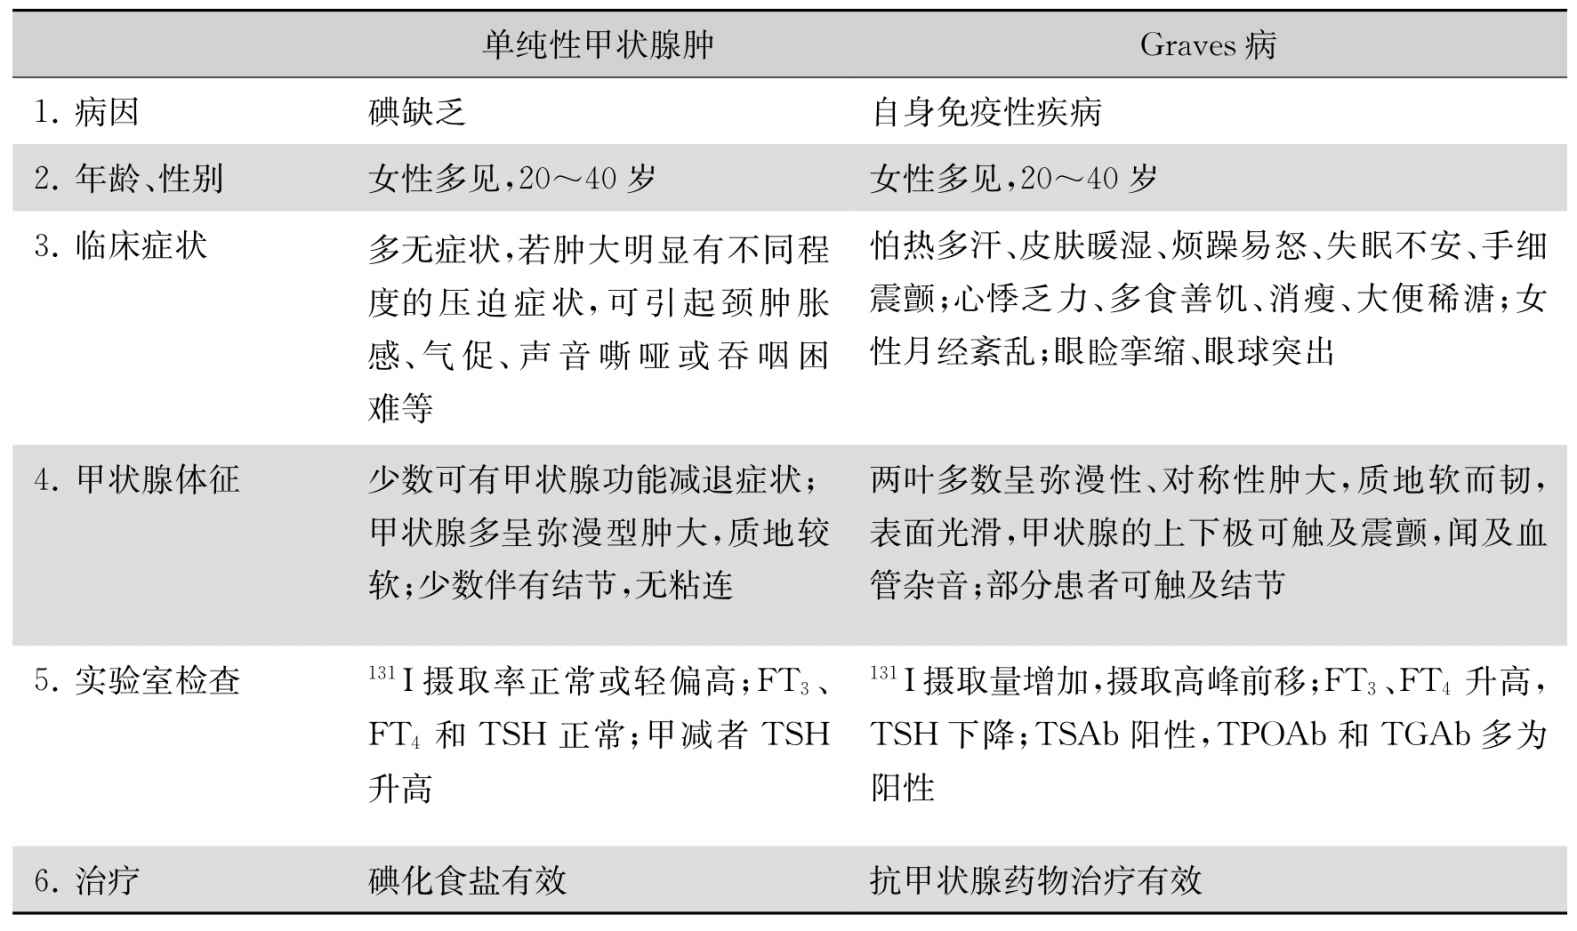
\includegraphics[width=5.90625in,height=3.47917in]{./images/Image00239.jpg}
\end{table}

\begin{table}[htbp]
\centering
\caption{甲状腺毒症的病因鉴别}
\label{tab38-3}
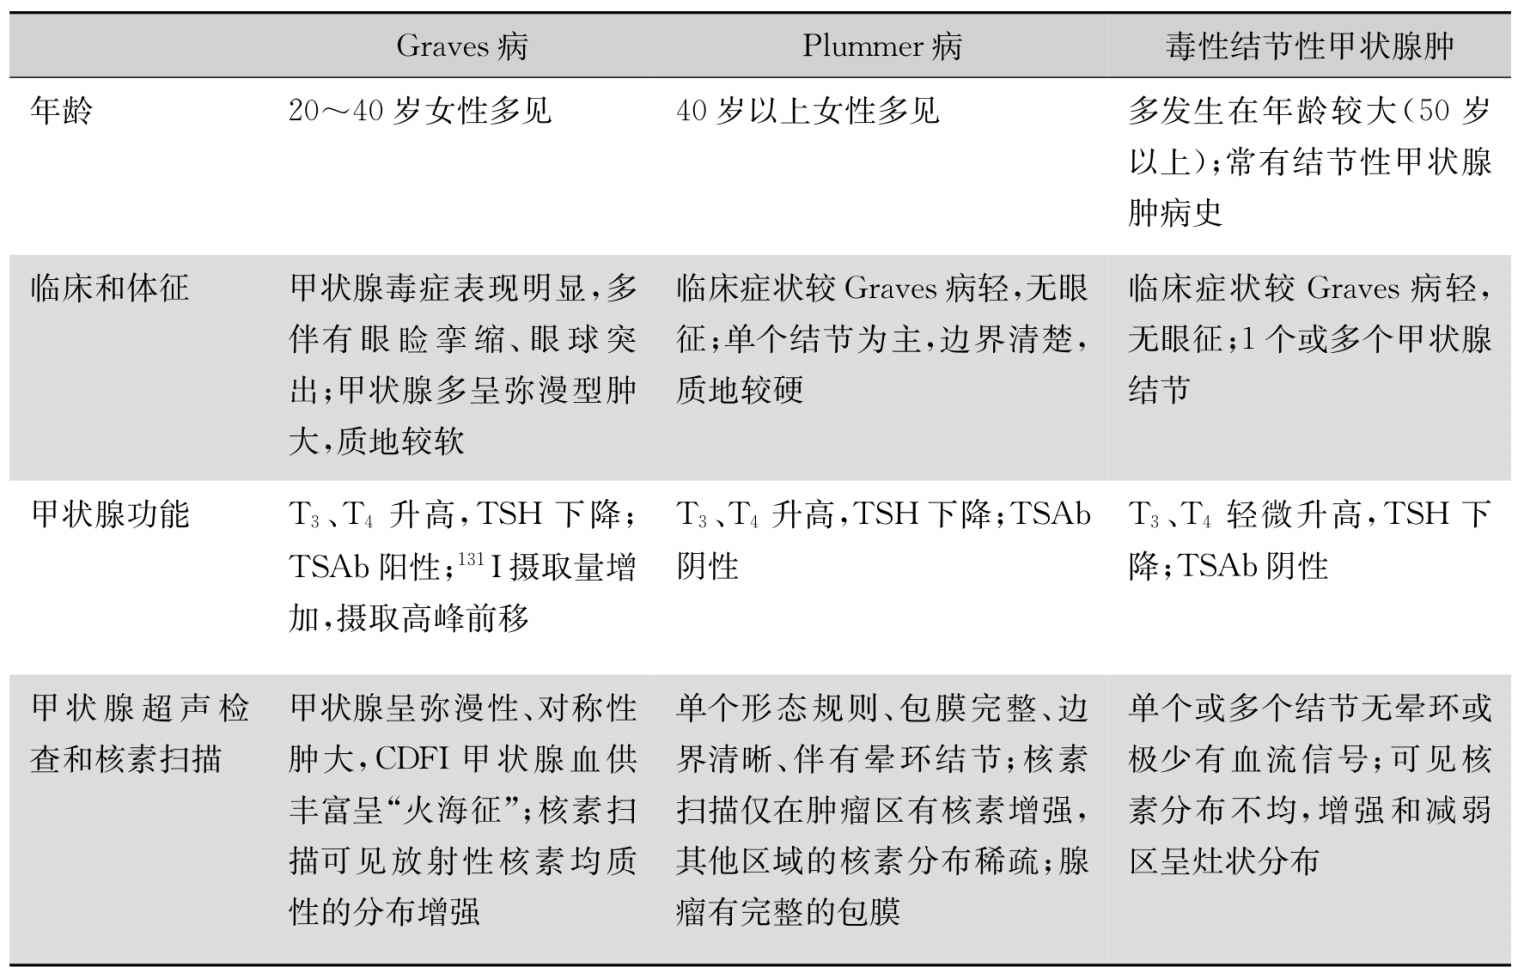
\includegraphics[width=5.90625in,height=3.77083in]{./images/Image00240.jpg}
\end{table}

\subsubsection{(六)Graves病与非甲状腺疾病的鉴别}

\paragraph{1.神经症}

有心悸、脉速、失眠焦虑等类似于甲亢的表现。但神经症患者一般无食欲亢进,也无甲状腺肿及突眼,甲状腺功能检查均为正常。

\paragraph{2.更年期综合征}

更年期妇女常有阵发性潮热、出汗,伴有情绪不稳定,烦躁失眠等症状,发作过后有怕冷。但其甲状腺不大,甲状腺功能基本正常。

\paragraph{3.消化系统疾病}

由于甲亢使肠蠕动增加,使大便稀溏、次数增加,临床上常易误诊为慢性结肠炎。但甲亢患者极少有腹痛、里急后重等肠炎表现,大便检查无炎症。也有少数患者伴恶心、呕吐,甚至出现恶病质以及肝功能异常等表现。在排除消化道器质性病变的同时应进行甲状腺功能的检测予以鉴别。

\paragraph{4.抑郁症}

老年人甲亢多为隐匿起病,表现为体虚乏力、精神忧郁、表情淡漠、原因不明的消瘦、食欲缺乏,恶心、呕吐等表现,与抑郁症相类似,测定甲状腺功能正常可以鉴别。

\paragraph{5.心血管系统疾病}

老年人甲亢常以心脏症状为主,如心房纤颤或心力衰竭,易被误诊为冠状动脉粥样硬化性心脏病。在甲状腺毒症患者中10\%~15\%可发生心房纤颤;在原因不明的心房纤颤中,10\%是由甲状腺毒症引起的。部分老年甲亢是以心房纤颤为首发临床表现,而其他的甲亢症状不典型,易被漏诊、误诊。测定甲状腺功能可以鉴别。

\paragraph{6.糖尿病}

糖尿病的“三多一少”症状与甲亢的食欲亢进、易饥相似,特别是少数甲亢患者糖耐量异常。糖尿病患者亦可出现高代谢症状,但患者无心悸、怕热、烦躁等症状,甲状腺一般不肿大,甲状腺功能正常有助于鉴别。也有少数糖尿病患者伴有甲亢,两种病同时存在。

\paragraph{7.其他}

以消瘦、低热为主要表现者,应注意与结核、癌症相鉴别。有些甲亢患者表现为严重的肌萎缩,应注意与原发性肌病鉴别。

\protect\hypertarget{text00300.html}{}{}

\subsection{三、外源性因素致甲状腺功能亢进症}

\subsubsection{(一)碘诱导的甲亢}

在缺碘地区,补充碘可使地方性甲状腺肿患者的甲状腺缩小,功能恢复。但在非缺碘区域,补充碘可诱发甲亢,某地区报道补碘后甲亢的发病率增加了7倍。无论碘的来源如何,只要血清碘化物的浓度升高到足以弥散进入甲状腺组织,就能使有自主功能的甲状腺组织过度合成和分泌甲状腺激素。尿碘中位数>300μg/L提示碘过量。在食物中除了富碘食物(紫菜、海带等)摄入过多使机体碘过量外,也有一些蔬菜,如生食大量胡萝卜、卷心菜、大豆、白菜、萝卜等,因含有致甲状腺肿物质,均能阻止甲状腺浓聚碘或使酪氨酸不能碘化,而引起甲状腺代偿性肿大。

\subsubsection{(二)甲状腺激素诱导的甲亢}

服用甲状腺激素剂量过大可引起甲亢,多见于长期服用甲状腺激素,尤其具有自主甲状腺功能的患者,较小剂量即可引起亚临床甲亢或临床甲亢。甲状腺肿瘤或结节性甲状腺肿患者用甲状腺激素治疗以抑制TSH,有时可发生甲亢。

\subsubsection{(三)药物诱导的甲亢}

胺碘酮的含碘量为37.2\%,当治疗剂量每日为300mg时,相当于服药者每日接受了100mg的碘量。胺碘酮对甲状腺功能的影响既有急性作用,也有慢性作用,它还能够抑制外周T\textsubscript{4}
向T\textsubscript{3}
的转化,引起甲状腺毒症的发生。另外,在用α-干扰素治疗的患者,约有2\%可发展为甲亢。

不适当的补碘是碘过量最常见的原因之一,即在碘充足地区补碘,或在碘缺乏地区过度补碘。碘过量导致的甲亢称碘性甲亢,碘甲亢的症状与一般甲亢基本相同,但患者年龄相对偏大,症状出现顺序往往是先出现神经、心脏症状,而后出现乏力、体重下降等。碘甲亢患者甲状腺可轻度肿大,质地较硬可触及结节,非缺碘地区结节性甲状腺肿患者补碘后发生甲亢的病例较多见。甲状腺部位无血管杂音和震颤,突眼少见,可有肌肉轻度萎缩。甲状腺摄131碘率降低为其特征,24小时摄\textsuperscript{131}
I百分率可低于30\%,甲状腺显像显影差,其他检查同一般甲亢。

\protect\hypertarget{text00301.html}{}{}

\subsection{四、甲状腺自主性高功能腺瘤(Plummer disease)}

又称Plummer病或毒性甲状腺腺瘤,多由于腺瘤细胞TSH受体的基因发生突变所致,毒性甲状腺腺瘤是直径≥3cm的孤立结节。以女性和40岁以上多见。临床多以颈部单个结节为主要症状,若腺瘤出血坏死时也可出现一过性甲亢。一般在诊断时有20\%患者有临床甲亢或亚临床甲亢,甲亢的程度较Graves病轻。颈部可触及圆形或卵圆形结节,边界清楚,质地较硬,随吞咽活动,无血管杂音。甲状腺功能T\textsubscript{3}
、T\textsubscript{4}
升高,TSH下降;甲状腺腺瘤超声声像图:一般为形态规则的圆形或椭圆形,有完整的包膜,边界清楚,周边大多有晕环,内部回声均匀,可为低回声、等回声或偏高回声;亦可因囊性变而呈伴有液化区的混合性回声;病灶以外的甲状腺组织回声正常。因此在回声正常的甲状腺组织中,如果显示单个形态规则的、包膜完整的、边界清晰的、伴有晕环,仅在周边显示血流信号或无血流信号的回声均匀或囊性变的结节灶,首先考虑为毒性甲状腺腺瘤。甲状腺核素静态显像有显著特征,可见结节处有放射性碘浓聚为有功能的“热结节”,其余的甲状腺组织几乎不摄碘,即表现为核素的分布稀疏。

\protect\hypertarget{text00302.html}{}{}

\subsection{五、结节性毒性甲状腺肿}

毒性结节性甲状腺肿也可发生甲亢,特别是年龄50岁以上的妇女,毒性结节性甲状腺肿的发展非常缓慢。典型患者具有甲状腺逐渐增大的病史以及隐匿发展的亚临床或临床甲亢。患者无眼征或局部黏液性水肿的甲状腺以外的表现。毒性结节性甲状腺肿患者可触及1个或多个甲状腺结节,有时甲状腺呈弥漫性肿大。患者中甲状腺肿大程度与甲亢的严重程度差异很大。

毒性结节性甲状腺肿的声像图:病理上结节性甲状腺肿是甲状腺增生的结果,无包膜、周围可被纤维组织厚薄不等、不完整地包绕。由于纤维组织压迫了间质中的血管,可因退行性变、坏死、出血等而囊性变。大多数结节性甲状腺肿的结节无晕环或极少有血流信号。甲状腺核素静态显像,毒性结节性甲状腺肿者可见核素分布不均,增强和减弱区呈灶状分布。

\protect\hypertarget{text00303.html}{}{}

\section{127 甲状腺炎}

甲状腺炎的病因不同,组织学特征各异,临床表现及预后差异较大。患者可以表现甲状腺功能正常、一过性甲状腺毒症或甲状腺功能减退症,有时在病程中这3种功能异常均可发生,部分患者最终发展为永久性甲减。甲状腺炎的分类:按发病的急缓可分为急性、亚急性及慢性甲状腺炎;按组织病理学可分为化脓性、肉芽肿性、淋巴细胞性、纤维性甲状腺炎;按病因可分为感染性、自身免疫性、放射性甲状腺炎等。其中无痛性甲状腺炎、慢性淋巴性甲状腺炎、产后甲状腺炎这三种甲状腺炎归为自身免疫性甲状腺炎(AIT)。

\subsection{一、急性化脓性甲状腺炎}

急性化脓性甲状腺炎比较罕见,以发热、甲状腺肿痛为特征。大多由化脓性细菌经血行或邻近感染蔓延至甲状腺所引起。起病急、伴有发热、畏寒;甲状腺肿大、疼痛、压痛,并向耳、颊、枕部放射,吞咽困难和疼痛加剧;局部压迫症状明显;甲状腺往往一侧肿大,质硬,但也可侵犯双侧,表面皮肤潮红水肿;后期脓肿形成时有波动感,可抽得脓液,涂片染色或培养可证明有化脓性细菌。实验室检查:白细胞明显升高及中性粒细胞增多,血沉增快;血清T\textsubscript{3}
、T\textsubscript{4}
一般正常;甲状腺B超可有液性暗区;甲状腺穿刺可抽出脓液。抗生素治疗或手术切开引流效果明显。

\subsection{二、亚急性甲状腺炎}

亚急性甲状腺炎(subacute thyroiditis)又称De
Quervain甲状腺炎,约占甲状腺疾病的5\%左右,以30~50岁女性最为多见。本病呈自限性,是最常见的甲状腺疼痛疾病。多由甲状腺的病毒感染(流感病毒、柯萨奇病毒、腮腺炎病毒以及腺病毒等)引起。常在病毒感染后1~3周发病:①上呼吸道感染前驱症状:发热、肌肉疼痛、咽痛、疲劳、倦怠等不适;②甲状腺区特征性疼痛:逐渐或突然发生,程度不等。转颈、吞咽动作时加剧,常放射至同侧耳、咽喉、下颌角、颏以及枕部等处,疼痛常先累及一叶后扩展到另一叶甲状腺;③甲状腺肿大:弥漫或不对称轻、中度增大,多数伴结节,质地较硬,触痛明显,无震颤及杂音。临床分期:①急性发作期:50\%~75\%患者伴有甲状腺毒症表现;②缓解期:部分患者出现功能减退症状;③恢复期:多数患者恢复正常,仅少数成为永久性甲减。整个病程约6~12个月,有些病例反复加重,持续数月至2年不等。

典型的实验检查结果是:甲状腺毒症期\textsuperscript{131}
I摄取率低而T\textsubscript{3} 、T\textsubscript{4}
增高的“分离现象”,随着甲状腺细胞的修复,摄碘功能逐渐恢复,缓解期可出现一过性甲减;而当炎症消退,血清T\textsubscript{3}
、T\textsubscript{4}
亦渐恢复正常。急性发作期患者的红细胞沉降率(ESR)明显增快,ESR>50mm/h对诊断有利;白细胞计数可增高。血清Tg水平明显增高,与甲状腺破坏程度相一致,且恢复很慢,但Tg不作为诊断必备的指标。CDFI显示甲状腺腺体内血流信号有增多现象。FNAC检查:早期典型细胞学涂片可见多核巨细胞、片状上皮样细胞、不同程度炎性细胞;晚期往往见不到典型表现。FNAC检查不作为诊断本病的常规检查。本病对糖皮质激素的治疗效果甚佳,能在短期内控制症状。

鉴别诊断要点:

\subsubsection{1.急性化脓性甲状腺炎}

甲状腺局部或邻近组织红、肿、热、痛及全身显著炎症反应,有时可找到邻近或远处感染灶;白细胞明显增高,核左移;甲状腺功能及摄碘率多数为正常。

\subsubsection{2.结节性甲状腺肿出血}

突然出血可伴甲状腺疼痛,出血部位伴波动感;但无全身症状,ESR不升高;甲状腺超声检查对诊断有帮助。

\subsubsection{3.桥本甲状腺炎}

少数病例可以有甲状腺疼痛、触痛,活动期ESR可轻度升高,并可出现短暂甲状腺毒症和摄碘率降低;但是无全身症状,血清TgAb、TPOAb滴度增高。

\subsubsection{4.无痛性甲状腺炎}

本病是桥本甲状腺炎的变异型,是自身免疫甲状腺炎的一个类型。有甲状腺肿,临床表现经历甲状腺毒症、甲减和甲状腺功能恢复3期,与亚急性甲状腺炎相似。鉴别点:本病无全身症状,无甲状腺疼痛,ESR不增快,必要时可行FNAC检查鉴别,本病可见局灶性淋巴细胞浸润。

\subsubsection{5.甲状腺功能亢进症}

碘致甲亢或者甲亢时摄碘率被外源性碘化物抑制,出现血清T\textsubscript{4}
、T\textsubscript{3} 升高,但是\textsuperscript{131}
I摄取率降低,需要与亚急性甲状腺炎鉴别。根据病程、全身症状、甲状腺疼痛、甲亢时T\textsubscript{3}
/T\textsubscript{4} 比值及ESR等方面可以鉴别。

\subsection{三、慢性淋巴性甲状腺炎(桥本甲状腺炎)}

慢性淋巴性甲状腺炎又称桥本甲状腺炎(HT)是常见的自身免疫性甲状腺疾病之一,其临床特征是无痛性、弥漫性甲状腺肿大,血清甲状腺自身抗体(TPOAb和TGAb)浓度高,50\%患者最终发生甲状腺功能减退。女性发病率是男性的3~4倍,甚至更高,高发年龄在30~50岁,且随年龄增加,患病率增高。此病常与其他自身免疫性疾病同时伴发。研究认为桥本甲状腺炎主要是Th1型细胞因子介导的细胞免疫反应起主要作用;TPOAb所介导的抗体依赖性细胞介导的细胞毒(ADCC)效应是导致已受损的甲状腺滤泡细胞被进一步破坏的重要机制。

1.临床表现
起病隐匿,进展缓慢,早期的临床表现常不典型。甲状腺肿大呈弥漫性、分叶状或结节性肿大,质地大多韧硬,与周围组织无粘连。常有咽部不适或有颈部压迫感,偶有局部疼痛。随病程延长,甲状腺组织破坏出现甲减症状,怕冷、心动过缓、便秘甚至黏液性水肿等。本病也可与Graves病并存,称为桥本甲状腺毒症(Hashitoxicosis)。临床表现为甲亢和甲减交替出现,可能与刺激性抗体或阻断性抗体占主导作用有关。甲亢的症状与Graves病类似,程度较轻,需正规抗甲状腺治疗,但治疗中容易发生甲减;也有部分患者为一过性甲状腺毒症。另外,HT还可同时伴有其他自身免疫性疾病。

2.实验室检查
甲状腺功能测定的结果与本病的病程相关可以分为3期,早期仅有甲状腺自身抗体阳性,血清FT\textsubscript{3}
、FT\textsubscript{4}
和TSH均是正常;随着病情的发展,血清TSH升高,FT\textsubscript{3}
、FT\textsubscript{4}
仍正常,表明甲状腺功能失代偿,出现了亚临床甲减;最后血清FT\textsubscript{3}
、FT\textsubscript{4}
水平均下降,进入临床甲减阶段。TPOAb和TGAb是最具有诊断意义的指标,尤其在出现甲减以前,抗体阳性是诊断本病的唯一依据。TPOAb的滴度与甲状腺淋巴细胞浸润的程度密切相关,TPOAb的阳性率(97\%)和滴度均高于TGAb(80\%)。当出现临床甲减时,\textsuperscript{131}
I摄取率降低。甲状腺超声显示:甲状腺肿大呈弥漫性、不均匀的低回声改变或甲状腺结节,若在低回声内还可见到网格样条索状强回声改变,此为桥本甲状腺炎所特有的超声显像,有鉴别诊断价值。甲状腺核素显像:可显示不规则浓集与稀疏,或呈“冷结节”改变。甲状腺细针穿刺细胞学检查(FNAC)镜下可见中度或大量淋巴细胞浸润,可形成滤泡和生发中心,滤泡上皮细胞肿胀增大,胞质丰富、呈嗜酸染色反应---Hürthle细胞。

桥本甲状腺炎需与结节性甲状腺肿和甲状腺癌进行鉴别:

1.结节性甲状腺肿
有地区流行病史,甲状腺功能正常,甲状腺自身抗体阴性或低滴度。FNAC检查有助鉴别。HT可见淋巴细胞浸润,少量的滤泡上皮细胞表现为Hürthle细胞的形态;结节性甲状腺肿则为增生的滤泡上皮细胞,没有淋巴细胞浸润。

2.甲状腺癌
甲状腺明显肿大,质硬伴结节者需要与甲状腺癌鉴别。但是分化型甲状腺癌多以结节首发,不伴甲状腺肿,抗体阴性,FNAC检查可见恶性病变;HT与甲状腺淋巴瘤的鉴别较为困难。

\subsection{四、产后甲状腺炎}

产后甲状腺炎(PPT)是发生在产后的一种亚急性自身免疫性甲状腺炎。妊娠时的免疫抑制状态保护作用在分娩后解除,诱发具有潜在甲状腺自身免疫倾向转变为临床形式。甲状腺自身抗体与PPT的相关性已得到公认,TPOAb阳性的妇女将有4\%~60\%发病,TPOAb阳性妇女发生PPT的危险性是TPOAb阴性妇女的20倍,所以TPOAb是预测妊娠妇女发生PPT的重要指标,若TPOAb阳性也说明患者存在潜在的AIT。过量的碘摄入是诱发PPT发生的因素,因此,在碘充足地区平均患病率约为7\%,国内学者报道PPT的患病率是11.9\%。

PPT可分为3个亚型,即甲亢甲减双相型、甲亢单相型和甲减单相型。临床PPT中甲亢甲减双相型占42.9\%,甲减单相型占11.4\%,甲亢单相型占45.7\%,甲亢甲减双相型是PPT典型的临床过程。①甲亢期:产后(通常在3个月)发生一过性甲亢,表现为心悸、乏力、怕热、情绪激动等症状,一般持续1~2个月;实验室检查特征性是血清T4、T3水平升高,甲状腺摄碘率显著降低呈现“双向分离”现象;②甲减期:通常在产后6个月左右发生,一般持续4~6个月,表现为肌肉、关节疼痛和僵硬,疲乏无力、注意力不集中、便秘等症状;血清TSH水平逐渐升高,甲状腺激素水平下降;③恢复期:经过自身修复,甲状腺功能恢复正常。但是约有20\%患者的甲减不能恢复,发展为永久性甲减。少数病例可以在PPT恢复后3~10年再发生甲减。PPT患者甲状腺轻、中度肿大,质地中等,但无触痛。超声检查显示低回声或低回声结节。FANC为轻度的淋巴细胞浸润,不形成生发中心,没有Hürthle细胞。

甲亢期需要与产后Graves病复发进行鉴别,主要有3个鉴别点:

(1)产后Graves病复发者常有产前的Graves病史或伴有Graves病特征性表现,如浸润性突眼等,甲亢的症状较重;而PPT产前无甲状腺功能异常病史。

(2)甲状腺摄碘率:甲亢期PPT减低;产后Graves病增高,但是受哺乳限制患者不能做此检查。

(3)TRAb:产后Graves病TRAb阳性,PPT则为阴性。

\subsection{五、无痛性甲状腺炎}

无痛性甲状腺炎(silent
thyroiditis)又称亚急性淋巴细胞性甲状腺炎,也是AIT的一个类型。本病甲状腺的淋巴细胞浸润较HT轻,表现为短暂、可逆的甲状腺滤泡破坏、局灶性淋巴细胞浸润,50\%患者血中存在甲状腺自身抗体。发病年龄以30~50岁为多,女性略多于男性。临床上半数患者的甲状腺轻度肿大,呈弥漫性,质地较硬,无结节,无血管杂音,无疼痛及触痛为其特征。1/3患者的甲状腺持续肿大。典型的甲状腺功能变化类似于亚急性甲状腺炎,分为3个阶段,即甲状腺毒症期、甲减期和恢复期。有50\%的患者不进入甲减期,甲状腺功能即可恢复正常。约40\%患者进入为期2~9个月的甲减期,其严重程度与TPOAb的滴度直接相关。若甲减期持续6个月以上,成为永久性甲减的可能性较大。10年后约20\%的患者存在持续性甲减,10\%~15\%者复发。

甲状腺摄碘率:甲状腺毒症阶段<3\%是重要的鉴别指标之一,恢复期甲状腺摄碘率逐渐回升。甲状腺毒症期血清T\textsubscript{3}
、T\textsubscript{4} 增高,T\textsubscript{3} /T\textsubscript{4}
比值<20对诊断有帮助;甲减期减低;恢复期逐渐降至正常。半数以上TgAb、TPOAb阳性,滴度比较高;少数存在TSAb或TSBAb。自身抗体阳性不作为必备诊断条件。Tg明显升高,可持续长达2年。甲状腺核素扫描显示甲状腺无摄取或摄取低下对诊断有帮助。FANC检查可见淋巴细胞浸润。

本病很难与无突眼、甲状腺肿大不显著的Grave病鉴别;后者病程较长,甲状腺毒症症状更明显,T\textsubscript{3}
/T\textsubscript{4}
比值往往>20,甲状腺摄碘率增高伴高峰前移。必要时可行FANC检查加以鉴别。

\subsection{六、慢性纤维性甲状腺炎}

慢性纤维性甲状腺炎又称Riedel甲状腺炎,是一种病因未明而罕见的甲状腺疾病,好发于成年女性,以甲状腺广泛纤维化、甲状腺功能减退和明显的压迫症状等为特征。一般认为Riedel甲状腺炎是全身纤维化的一部分,如可伴有纤维性胆道炎、局灶性肺纤维化、腹膜后纤维化、眼眶后纤维化以及纵隔纤维化等。甲状腺中度肿大,常为单侧,十分坚硬,与周围组织粘连;多数出现明显的压迫症状,如压迫气管引起呼吸困难,压迫食管则有吞咽障碍,压迫喉返神经表现为声音嘶哑等。约30\%患者出现甲状腺功能减退;影像学检查可见甲状腺肿大,周围组织粘连;甲状腺穿刺活检可见典型的组织纤维化和不同程度的细胞浸润。外科手术可解除压迫症状。

\protect\hypertarget{text00304.html}{}{}

\section{128 甲状腺结节}

在临床甲状腺结节十分常见,流行病资料显示,其罹患率在青少年约为1.5\%,随着年龄的增高,成人约为4\%,60岁以上人群约为5\%。触诊发现一般人群甲状腺结节的患病率为3\%~7\%,随着健康检查的普及,甲状腺超声作为常规的检查项目,大大提高了甲状腺结节的罹患率。超声检查的发现率达20\%~70\%。甲状腺结节多为良性,恶性结节仅占5\%左右,因此,甲状腺结节诊治的关键是鉴别良、恶性。

甲状腺结节在不同检查方法中的表现不同,如触诊发现的甲状腺结节为甲状腺区域内扪及的肿块;而超声检查发现的甲状腺结节为局灶性回声异常的区域。这两种检查方法的结果有时会不一致,如体检时扪及到了甲状腺肿块,但甲状腺超声并没有发现结节;或体检时没有触及甲状腺结节,而超声检查却有甲状腺结节的存在。

在确认甲状腺结节后,应鉴别结节的良、恶性,病史和体检对鉴别诊断有很大帮助。其中年龄是一个重要因素,15岁以下的患者甲状腺单个结节中20\%~50\%是恶性的,但大多为分化好的甲状腺癌。中老年的甲状腺癌发病率比较高,特别是未分化癌多在60岁以上。其次是性别与甲状腺癌的病理类型有关,乳头状甲状腺癌好发于年轻女性,而髓样癌和未分化癌则多发于男性。另外,要注意甲状腺肿瘤有较明显的家族遗传史。甲状腺结节的病因分类见表\ref{tab38-4}。

随着高分辨率全数字化超声仪和高频探头的使用,超声检查已经可以发现小于2mm的肿块,结合彩色多普勒血流成像技术,是目前评价甲状腺结节最敏感的方法。超声检查不但可以探测甲状腺结节的形态、大小、数目,更重要的是可以判别结节的性质,囊性或实质性,肿瘤有无包膜、周围的血流情况。如图像呈现光点分布均匀,光带清楚,边界整齐,囊腔内无明显乳头,大多数为良性结节;如表现为结节不均质,结节无明显包膜,结节包膜血流丰富呈“火焰山”样变化,加上有砂粒样的钙化灶,要注意癌的可能性较大。在甲状腺癌患者手术前和手术后复查,超声检查颈淋巴结有无肿大极为重要。此外,还可用于超声引导下甲状腺细针穿刺和细胞学的检查。超声诊断已成为甲状腺结节诊断的主要检测手段。

甲状腺放射性核素扫描:大约90\%的甲状腺癌其摄碘功能低下,良性结节的摄碘率多在正常范围内。根据甲状腺结节对放射性核素摄取的情况分4种类型:①热结节:多见于滤泡型腺癌、毒性腺瘤;②温结节:多见于腺瘤、结节性甲状腺肿;③凉结节:甲状腺囊肿最多见,其次为甲状腺癌、淋巴细胞性甲状腺炎、慢性纤维性甲状腺炎;④冷结节:单个实质性甲状腺肿瘤,约有50\%有癌变的可能。

甲状腺细针穿刺细胞学检查(FNAC):FNAC对术前甲状腺结节的评估比核素扫描、生化检测等方法准确性高。FNAC对良性结节的诊断比较可靠,假阴性率在1.3\%~11.8\%,主要发生在囊性结节较多。细胞学诊断假阳性率较低,国内一组报道为0.8\%。FNAC也有一定的局限性,缺乏对整体组织结构的了解。FNAC可确认甲状腺滤泡肿瘤,但缺乏明确的良性或恶性的特征,无法区别滤泡状腺瘤或滤泡样腺癌,因为后者一定要有包膜的侵袭才能作出诊断。

\begin{table}[htbp]
\centering
\caption{甲状腺结节的分类及病因}
\label{tab38-4}
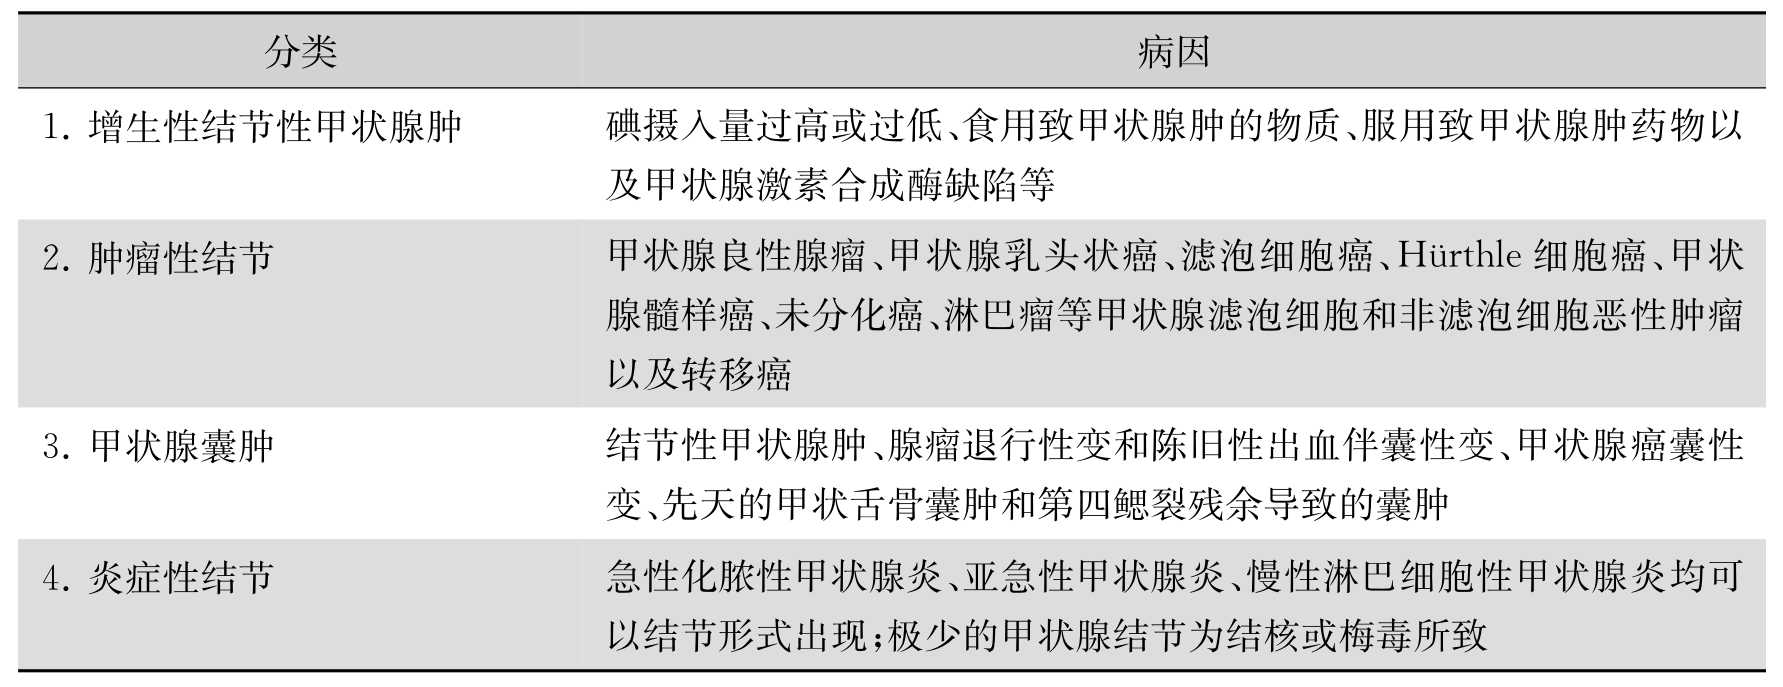
\includegraphics[width=5.9375in,height=2.28125in]{./images/Image00241.jpg}
\end{table}

\subsection{一、甲状腺良性结节}

绝大多数甲状腺结节患者没有临床症状,通常是通过体检或触摸或影像学检查而发现的。当肿大结节压迫周围组织时,可出现相应的临床表现,如声音嘶哑、憋气、吞咽困难等。详细的病史采集及检查对于评估甲状腺结节的性质很重要。病史采集的要点是患者的年龄、性别、有无头颈部放射线检查或治疗史;结节的大小及变化和增长的速度、有无局部症状、有无甲亢或甲减的症状;有无甲状腺肿瘤等家族性疾病史。体格检查的重点是结节的数目、大小、质地、活动度、有无压痛、有无颈部淋巴结肿大等。

\subsubsection{(一)甲状腺腺瘤}

多见于20~40岁的女性,病灶大多为单发结节,较少多发,累及两叶,肿瘤生长缓慢。多无自觉症状,无意中发现或体检时发现。甲状腺腺瘤均来自甲状腺滤泡上皮。一般为单发的圆形或椭圆形肿物,直径多在1~5cm,包膜完整,质柔韧,与周围组织分界清楚,多并发囊性变。根据病理形态分为:①滤泡状腺瘤;②胚胎型腺瘤;③胎儿型腺瘤;④嗜酸性腺瘤;⑤乳头状腺瘤和乳头状囊腺瘤;⑥不典型腺瘤。以滤泡状腺瘤最多见,少数较大腺瘤者可有压迫症状。

\subsubsection{(二)结节性甲状腺肿}

初期为双侧甲状腺弥漫性肿大,后期可产生结节,常为多个大小不一,质韧或较软,表面光滑,随吞咽上下活动。部分病例可合并甲状腺功能亢进,少数可发生癌变。由于结节性甲状腺肿呈双叶多发性结节生长,单纯手术摘除效果不佳,极易复发。国内一组4899例结节性甲状腺肿的数据显示,男性占15.9\%,女性为84.1\%。

\subsubsection{(三)结节性甲状腺肿与甲状腺腺瘤的鉴别}

结节性甲状腺肿和甲状腺腺瘤都表现为颈部甲状腺部位的肿块或结节,理论上不难鉴别,临床实际则不然。国内报告一组4453例结节性甲状腺肿,术前正确诊断率71.95\%。误诊的病例绝大多数是结节性甲状腺肿误诊为甲状腺腺瘤,而甲状腺腺瘤误诊为结节性甲状腺肿者仅占甲状腺腺瘤总数的3.75\%。一般查体触诊结节性甲状腺肿为甲状腺整体不均匀性肿大,而甲状腺腺瘤则为甲状腺肿大的结节。触诊时肿大的结节最明显也易扪及,查体往往忽略了对侧甲状腺和结节同侧周围甲状腺的情况,或把周围甲状腺和结节一起判断为一个较大的结节,是诸多结节性甲状腺肿被误诊为甲状腺腺瘤的原因之一。

其次,2个以上结节的多为结节性甲状腺肿,单个结节既可能是甲状腺腺瘤,也可能来自结节性甲状腺肿。在4899例结节性甲状腺肿组的数据分析中,双侧病变为84.9\%,单侧为15.1\%,双侧结节性甲状腺肿远高于单侧病变,说明结节性甲状腺肿的发生始于甲状腺的弥漫性病变,与其病理学发展过程相符。如果超声显示多结节,一般提示为结节性甲状腺肿,特别是双侧甲状腺有结节或一侧为多发结节,另一侧甲状腺组织回声不均时。若声像图为单个结节,周围甲状腺和对侧甲状腺组织回声均匀则提示甲状腺腺瘤。而相对于结节内部的回声、结节及其周围血流情况对结节性甲状腺肿或甲状腺腺瘤的鉴别诊断价值不是太大。

结节有无包膜在甲状腺腺瘤和结节性甲状腺肿鉴别诊断中也很重要,甲状腺腺瘤有完整包膜,而结节性甲状腺肿的结节界限清,一般无包膜或不完整。包膜不完整的良性甲状腺结节诊断为结节性甲状腺肿一般不会混淆,而对包膜较完整的结节的诊断却存在误区,易造成甲状腺瘤的过诊断。甲状腺瘤的纤维包膜完整,厚薄较一致,无挤压的甲状腺滤泡;而结节性甲状腺肿的包膜虽完整,但厚薄不均,可见多少不等的挤压甲状腺滤泡存在。

结节性甲状腺肿和甲状腺腺瘤皆可囊性变,或伴发出血,如短期明显增大的甲状腺结节,甚至出现胀痛不适,在超声检查排除了实性结节后,应考虑为结节囊性变伴出血。结节性甲状腺肿和甲状腺腺瘤的囊变率有非常显著的差异,结节性甲状腺肿的囊性变发生率高。因为一般甲状腺瘤体积较大时才发生囊性变,甲状腺腺瘤直径若小于1.5cm者不易发生囊性变;而结节性甲状腺肿囊性变则不分大小均可发生。因此可以认为,若小结节发生了囊性变,提示结节性甲状腺肿的结节可能,而非甲状腺腺瘤。

另外,结节性甲状腺肿有的和慢性淋巴细胞性甲状腺炎伴存,且多表现为局灶性淋巴细胞性甲状腺炎,甲状腺腺瘤则无局灶性淋巴细胞性甲状腺炎。因此,有无局灶性淋巴细胞性甲状腺炎可以作为结节性甲状腺肿和甲状腺腺瘤的鉴别点之一。结节性甲状腺肿与甲状腺腺瘤的鉴别参见表\ref{tab38-5}。

\begin{table}[htbp]
\centering
\caption{结节性甲状腺肿与甲状腺腺瘤的鉴别}
\label{tab38-5}
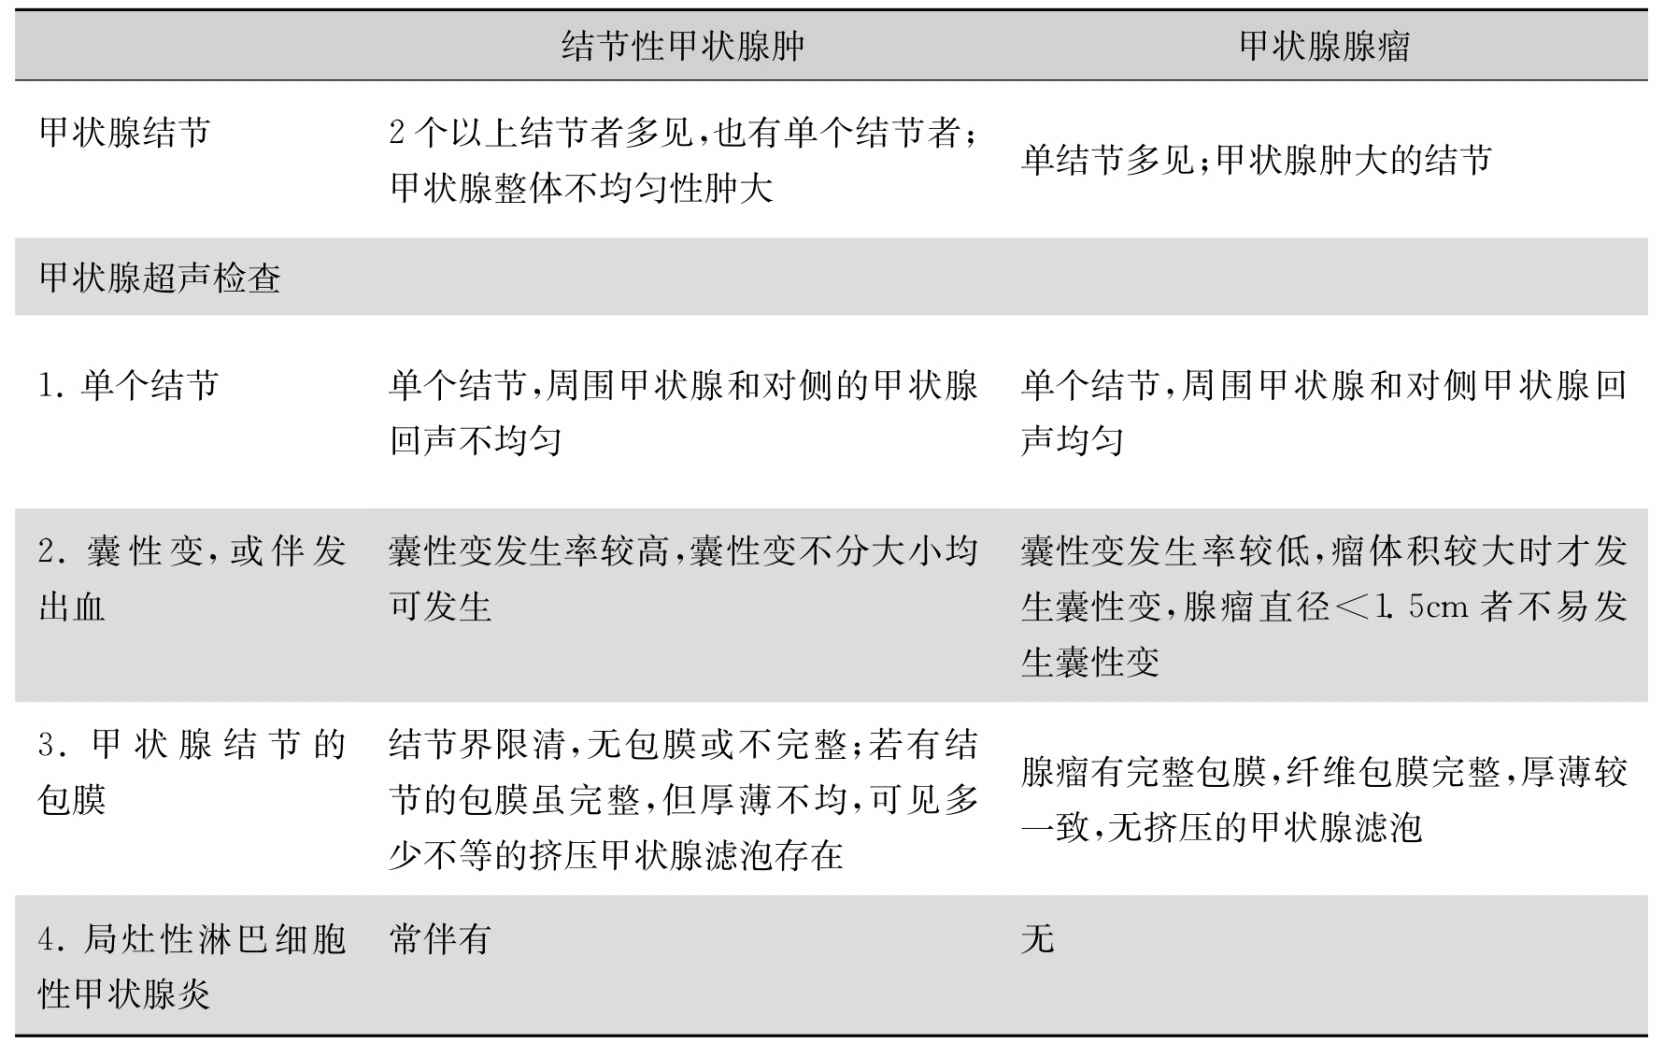
\includegraphics[width=5.92708in,height=3.76042in]{./images/Image00242.jpg}
\end{table}

\subsubsection{(四)甲状腺结节良、恶性的鉴别}

甲状腺超声检查确认甲状腺结节,再进行结节良、恶性的鉴别。高频超声检查甲状腺,能够准确、清晰地显示甲状腺结节的边界、内部结构以及对周围组织的浸润和颈部淋巴结的转移情况。虽然超声检查还不能准确区分良、恶性肿瘤,但可以提供有参考价值的信息。提示甲状腺结节恶性病变的特征有:①微小钙化;②结节边缘不规则;③结节内血流紊乱;这3项提示恶性病变的特异性高,均达80\%以上,但敏感性却不高,在29\%~77.5\%。因此,只有其中1项符合者不足以诊断恶性病变;如果同时存在2种以上特征时,或低回声结节中合并上述任何1项时,诊断的敏感性就能提高到87\%~93\%。微小钙化是恶性病灶的特有表现,基本等同于病理上的沙砾体,是诊断甲状腺癌的依据。另外,当低回声结节侵犯到甲状腺包膜外或甲状腺周围的肌肉中或颈部淋巴结肿大,伴淋巴结门结构消失、囊性变,或淋巴结内出现微小钙化,血流信号紊乱时提示结节为恶性。值得警惕的是,研究结果显示,结节的良、恶性与结节的大小无关,直径小于1.0cm的结节中,恶性并不少见;与结节是否可触及无关;与结节单发或多发无关;与结节是否合并囊性变无关。甲状腺结节良、恶性超声检查的鉴别详见表\ref{tab38-6}。

\begin{table}[htbp]
\centering
\caption{甲状腺结节超声检查声像图的鉴别}
\label{tab38-6}
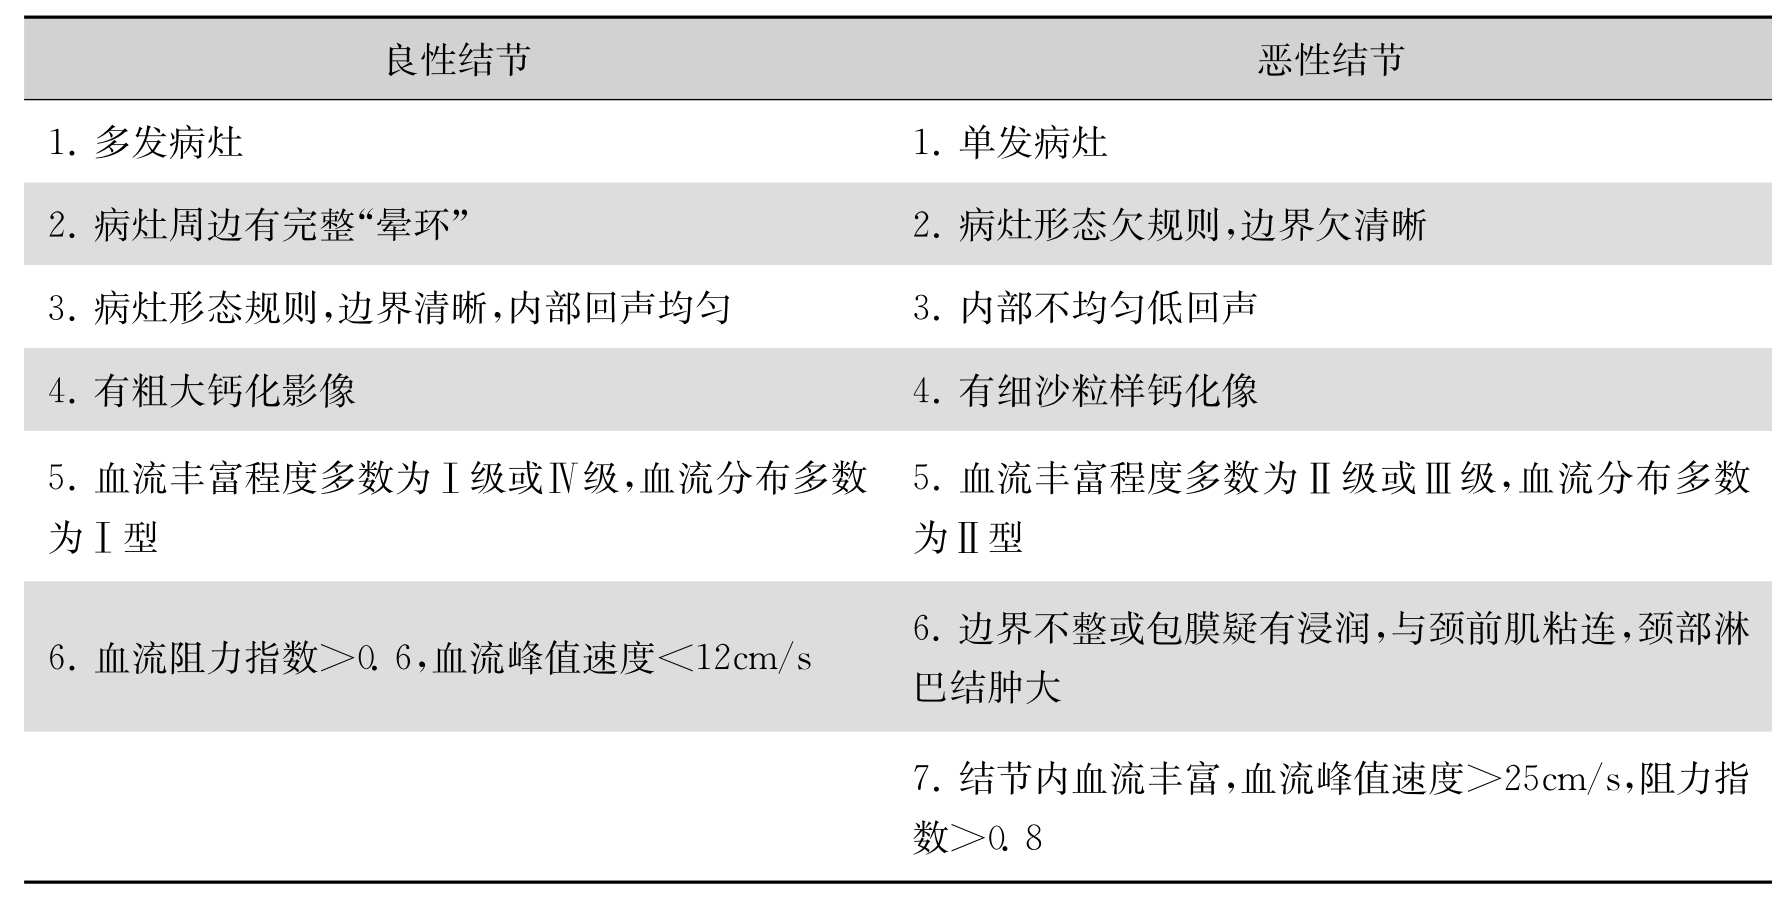
\includegraphics[width=5.95833in,height=3.01042in]{./images/Image00243.jpg}
\end{table}

甲状腺核素显像:其特点是能够评价甲状腺结节的功能。依据结节对放射性核素摄取能力将结节分为“热结节”、“温结节”和“冷结节”,其中“热结节”占10\%,“冷结节”占80\%。“热结节”中99\%为良性的,恶性者极为罕见;而“冷结节”中恶性率只有约5\%~8\%。因此,如果甲状腺核素显像为“热结节”者,几乎可以判断为良性;而通过“冷结节”来判断甲状腺结节的良、恶性则帮助不大。例如当结节囊性变或甲状腺囊肿者,若行甲状腺核素显像也表现为“冷结节”,此时,应结合甲状腺超声检查有助于诊断。

MRI和CT检查:MRI或CT对帮助发现甲状腺结节、判断结节的性质不如甲状腺超声检查敏感,且价格昂贵,故不推荐常规使用。但其对评估甲状腺结节和周围组织的关系,特别是发现胸骨后甲状腺肿有诊断价值。

FNAC检查:FNAC检查是鉴别结节良、恶性最可靠、最有价值的诊断方法,文献报道其敏感性达83\%,特异性达92\%,准确性达95\%。怀疑结节恶性变者均应进行FNAC检查。术前FNAC检查有助于术前明确癌症的细胞学类型,确定正确的手术方案。但FNAC检查不能区分甲状腺滤泡状癌和滤泡细胞腺瘤。

甲状腺恶性肿瘤患者绝大多数甲状腺功能正常;如果血清TSH减低,甲状腺激素增高,提示为高功能结节,此类结节绝大多数为良性。TPOAb和TgAb是检测桥本甲状腺炎的金指标之一,特别是血清TSH水平增高者。85\%以上桥本甲状腺炎患者,血清抗甲状腺抗体水平升高;但是少数桥本甲状腺炎可合并甲状腺乳头状癌或甲状腺淋巴瘤。

\subsection{二、甲状腺癌}

甲状腺癌约占全部恶性肿瘤的1\%,其发病的性别差异较大,通常女性为男性的2~4倍,不同类型的甲状腺癌的发病年龄高峰不同,乳头状癌多在30~39岁,滤泡状癌多见30~49岁,未分化癌则多见于70岁以上患者。提示甲状腺恶性结节临床证据包括:①有颈部放射线治疗史;②有甲状腺髓样癌或MEN2型家族史;③年龄小于20岁或大于70岁;④男性;⑤结节增长迅速,且直径超过2cm;⑥伴持续性声音嘶哑、发音困难、吞咽困难和呼吸困难;⑦结节质地硬、形状不规则、固定;⑧伴颈部淋巴结肿大。甲状腺恶性肿瘤患者绝大多数甲状腺功能正常。血清Tg对鉴别甲状腺结节的性质没有帮助,但可根据Tg水平的动态变化,监测分化型甲状腺癌手术治疗是否彻底,或术后甲状腺癌是否复发。如术后患者的Tg水平进行性升高,说明肿瘤的复发。降钙素是甲状腺髓样癌的肿瘤标志物,用于对甲状腺髓样癌进行诊断和术后随访的监测。有甲状腺髓样癌家族史或多发性内分泌腺瘤病家族史者,应检测基础或刺激状态下血清降钙素水平。

\subsubsection{(一)乳头状癌}

是一种分化好的甲状腺癌,也是最常见的一种,国内外文献报道约占78\%~82\%。病灶一般是单发,亦可发生在两叶或峡部,大小不等。好发于青、中年女性,因肿瘤生长缓慢,多在2~3年,少数达10余年。患者多无自觉不适的感觉,大部分除在甲状腺区域有一无痛性肿块外,很少有其他症状。一般活动度尚好,瘤体小于1cm者,多坚硬难以触及,常以淋巴结转移为主诉而就诊。瘤体较大时,直径可达10cm以上,常伴有囊性改变,穿刺可抽出黄棕色液体,易误诊为囊肿。晚期可累及周围组织出现压迫症状。典型的甲状腺乳头状癌常伴有同侧颈部淋巴结转移,约为50\%~70\%转移率,4\%的病例可转移至对侧颈部淋巴结。转移淋巴结的第一站往往是喉返神经区或气管前(中央区淋巴结),然后转移至颈侧区。常采用以下方法进行筛选:根据病史、体检疑有癌变者,结合超声检查,提示肿瘤无包膜,周围血流丰富,伴有微小钙化,辅以核素扫描提示“凉结节”或“冷结节”者,应实施手术探查。FNAC是最为方便的筛选方法,有条件的可常规使用。另外,颈部淋巴结的活检也有助于诊断。

\subsubsection{(二)滤泡状癌}

约占13\%~15\%,据WHO组织病理分类将Hürthle细胞癌列入滤泡状癌。发病年龄30~50岁,以颈前肿块就诊,一般病程较长,生长缓慢,常缺乏明显的局部恶性表现,单发多见,少数可双侧或多灶性,仅20\%发生淋巴结转移;常见主要是血行转移至肺和骨,有时患者以骨折就诊时被发现。转移的癌组织分化良好。本病主要靠病理确诊,用单克隆抗体MoAb-47对肿瘤进行过氧化物酶免疫组化的鉴别。由于滤泡状癌具有摄碘功能,如果合并有远处转移灶可再作\textsuperscript{131}
I治疗。

\subsubsection{(三)髓样癌}

发生于甲状腺滤泡旁细胞(C细胞)的恶性肿瘤,发生率3\%~10\%,临床以散发型为主(80\%以上),少数为家族性。C细胞的特征为分泌降钙素及癌胚抗原(CEA),并产生淀粉样物等。肿瘤大小不一,呈实质性,局限而硬,包膜多不完整,偶有钙化。颈前肿物多生长缓慢,病程较长。散发型髓样癌的临床表现同一般的甲状腺癌相似,发病年龄在50岁左右,肿瘤多为单发。家族型的发病年龄较年轻,20岁或之前,病变常为双侧,颈部淋巴结转移较多见。

家族型可分为:①多发性内分泌瘤(MEN)2A型:多合并单或双侧嗜铬细胞瘤和甲状腺旁腺亢进症,多有家族史;②MEN-2B型:合并嗜铬细胞瘤以及多发性黏膜神经瘤、Marfan体型,为常染色体显性遗传疾病。发生转移者还可伴顽固性腹泻,并出现类癌综合征;③家族性甲状腺髓样癌(FMCT):只有甲状腺髓样癌,呈家族性发病,不伴其他内分泌腺肿瘤。降钙素为本病具有诊断性的标志物,CEA升高都有助于鉴别诊断。RET癌基因突变的检测,中山大学附属第一医院内分泌科对MEN-2A的家系进行检测,结果显示在RET癌基因外显子11存在C634突变和D631的缺失,导致遗传性MEN-2A的发病。

\subsubsection{(四)未分化癌}

高度恶性肿瘤,约占3\%左右,好发于高龄男性,多数就诊时病灶已广泛浸润和远处转移。发病前常有甲状腺结节,肿块于短期内急骤增大,发展迅速,形成双侧弥漫性甲状腺巨大肿物,质硬、固定,广泛侵犯邻近组织,常以呼吸困难就诊,伴疼痛、声音嘶哑或吞咽不畅等压迫症状。本病甚难控制、预后极差。

\subsection{三、甲状腺肿瘤免疫组化指标的评估}

甲状腺过氧化物酶(TPO)在所有分化良好的甲状腺滤泡细胞上表达,是良性病灶的标志,对于鉴别良、恶性肿瘤有很高的特异性和准确性。半乳糖凝集素-3(Galectin-3):Galectin-3与肿瘤的侵袭、转移相关,在甲状腺癌尤其是乳头状癌中的表达,并随着肿瘤的进展程度它的表达水平越高,因而成为辨别甲状腺乳头状癌的一个标志物。细胞角蛋白19(CK19):CK19在甲状腺乳头状癌(包括滤泡型乳头状癌)中呈强阳性表达,有助于滤泡型乳头状癌、滤泡性腺癌和滤泡癌的鉴别。人骨髓内皮细胞(HBME-1):HBME-1在大部分乳头状癌和滤泡癌中高表达,而在结节性甲状腺肿、良性肿瘤中不表达。

上述是与甲状腺恶性肿瘤相关的、报道应用最广泛的免疫组化标记物,是甲状腺结节的良、恶性鉴别的免疫组化指标。有学者指出将这些指标进行组合、联合应用,可以明显提高恶性肿瘤的检出效率,其中以HBME-1和TPO的联合检测得到的准确性最高。当然,对甲状腺恶性肿瘤还可以进行包括:原位癌基因、抑癌基因、转移相关基因的突变等以及相关microRNA的检测进行诊断。

\protect\hypertarget{text00305.html}{}{}

\section{参考文献}

1.陈家伦.临床内分泌学.上海:上海科学技术出版社,2011:277-447

2.廖二元.内分泌学.第2版.北京:人民卫生出版社,2004

3.中国甲状腺疾病指南------甲状腺疾病的实验室及辅助检查.中华内科杂志,2007,46(8):697-702

4.Guan H,et al.High iodine intake is a risk factor of post-partum
thyroiditis:result of a survey from Shenyang,China.J Endocrinol
Invest,2005,28(10):876-881

5.中国甲状腺疾病指南------甲状腺功能亢进症.中华内科杂志,2007,46(10):876-882

6.Davies TF,et al.Thyrotixicosis//Williams Textbook of
Endocrinology.10th ed.Philadelphia:Saunders,2002:374-424

7.陈祖培,等.碘与甲状腺疾病//白耀.甲状腺病学.上海:科学技术文献出版社,2003:567-629

8.Teng W,et al.Effect of iodine intake on thyroid disease in China.N
Engl J Med,2006,354:2783-2793

9.中国甲状腺疾病指南------甲状腺炎.中华内科杂志,2008,47(9):784-788

10.李晨阳,等.碘摄入量对产后甲状腺炎发生、发展的影响.中华内分泌代谢杂志,2005,21(2):103-105

11.滕卫平.甲状腺炎//叶任高.内科学.第6版.北京:人民卫生出版社,2005,739-742

12.Hundahl SA,et al.A national cancer data base report on 53,856cases
of thyroid carcinoma treated in the
U.S.,1985-1995.Cancer,1998,83(12):2638-2648

13.中国甲状腺疾病指南------甲状腺结节.中华内科杂志,2008,47(10):867-868

14.Cooper DS,et al.Management guidelines for patients with thyroid
nodules and differentiated thyroid
cancer.Thyroid,2006,16(2):109-142

15.房学东,等.4453例结节性甲状腺肿临床分析.中华普通外科杂志,2003,18(8):494-495

16.Griffith OL,et al.Biomarker panel diagnosis of thyroid cancer:a
critical review.Expert Rev Anticancer Ther,2008,8(9):1399-1413

17.李文惠,等.结节性甲状腺肿和甲状腺腺瘤的鉴别诊断.现代肿瘤医学,2007,15(8):1086-1088

18.Yao B,et al.A novel mutation D631del of the RET gene was associated
with MEN-2Ain a Chinese pedigree.Endocr J,2009,56(1):99-104

19.Rodrigues,HG.,et al.Use of molecular markers in samples obtained
from preoperative aspiration of thyroid.Endocrine
J,2012,59(5):417-424

20.Yu S,et al.Circulating microRNA profiles as potential biomarkers for
diagnosis of papillary thyroid carcinoma.J Clin Endocrinol
Metab,2012,97(6):2084-2092

\protect\hypertarget{text00306.html}{}{}

